\section{Smart Grid}
\label{sec:smartgrid}
%\fbox{Responsible: RJP, Provisional date: Beginning ?}

\subsection{Example Description}
\label{sec:smartgrid_desc}

A smart grid is an electricity power grid where integrated ICT systems play a role in the control and management of the electricity power supply. 
\fbox{cite?}
Such ICT elements include distributed control in households, control of renewable energies and networked communications. 

In this section we outline a \SG\ model to explore different design decisions in the cyber control of an electricity power grid. The model presented here is a small illustrative example, which omits complexities of a real \SG. For example, the change from three-phase AC power to one-phase DC power allowing us to use simpler physical models. A second simplification is in the number of houses present in the grid model. We model only five houses, assumed to be in a small local area supplied by a single substation. We do not consider the remainder of the grid. To ensure that any effect due to changes in the power consumption by those properties are observed by the other houses, we skew the resistance of the transmission lines between the power generation and substation, and substation to houses. 


\subsection{Usage}
\label{sec:smartgrid_usage}

This is a work-in-progress pilot (available at \url{https://github.com/into-cps/case-study\_smart\_grid}) and not currently intended to be used for co-simulation; the \emph{master} branch therefore contains no models or FMUs. The work-in-progress artefacts are available in the \emph{development} branch. There are several subfolders for the various elements: \texttt{FMU} -- contains the various FMUs of the study; \texttt{Models} -- contains the in development constituent models defined using the INTO-CPS simulation technologies; \texttt{Multi-models} -- contains the multi-model definitions and co-simulation configurations; and \texttt{SysML} -- contains the SysML models defined for the study. 

\subsection{INTO-CPS SysML profile}
\label{sec:smartgrid_into_sys}

The SysML model of the \SG\ comprises an Architectural Structure Diagram (ASD) and a single Connections Diagram (CD). The ASD in Figure~\ref{fig:asd_1h}, shows that the multi-model is composed of four EComponents: \emph{FiveHouseGrid},  \emph{SubstationController},  \emph{DataNetwork} and  \emph{HouseController}. We model one CT physical element -- the grid itself -- in 20-sim, and three DE models for the ICT control and communication features.

\begin{figure}[htbp]
\begin{center}
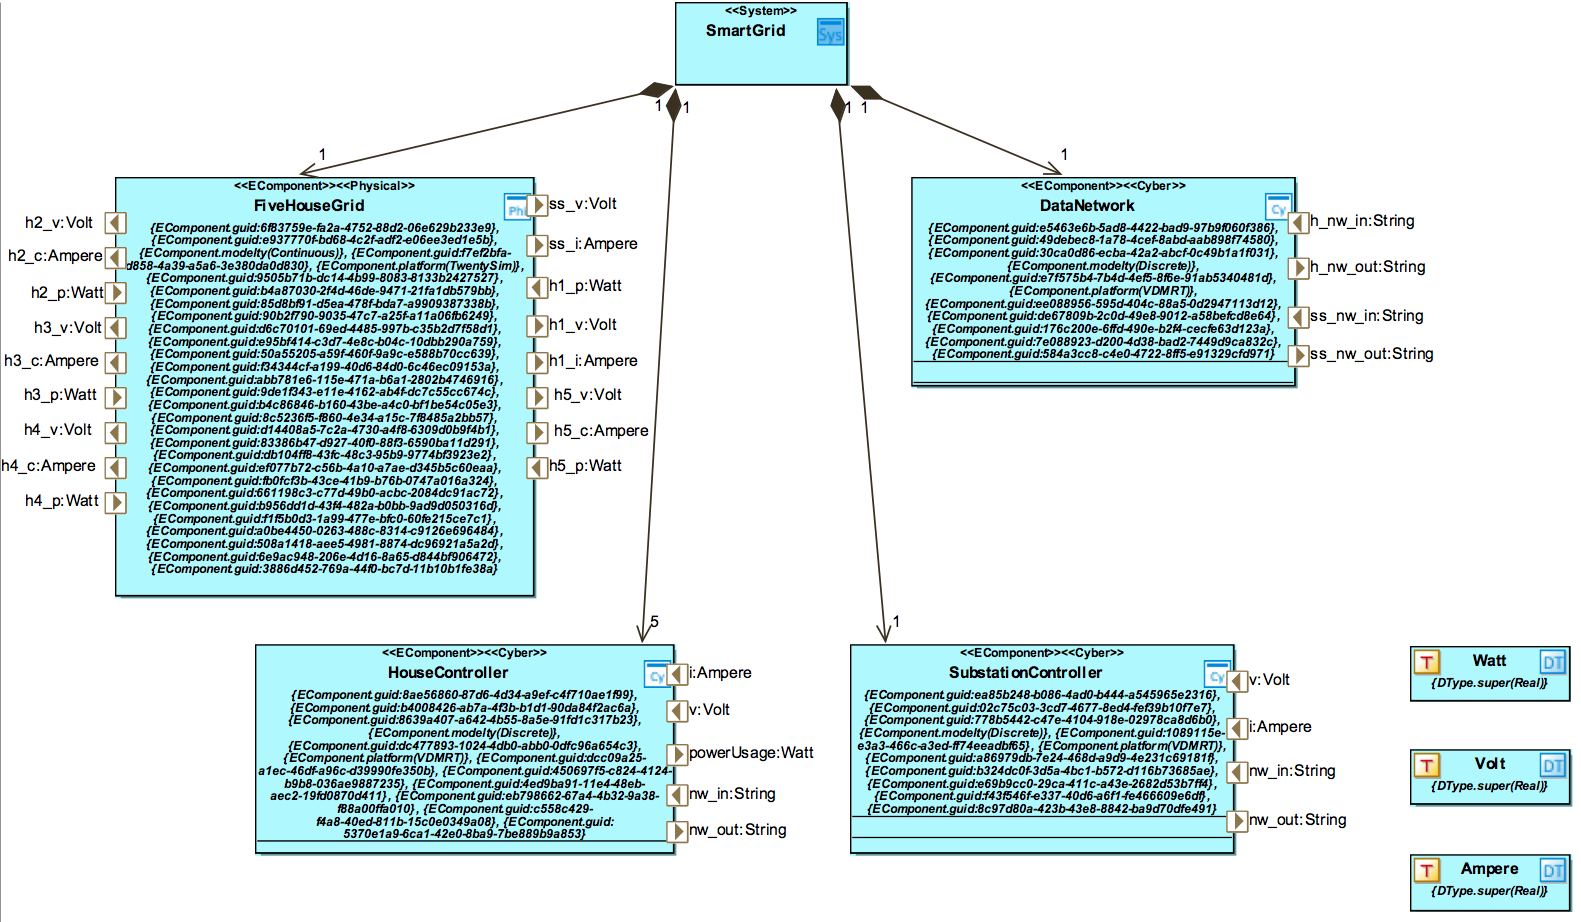
\includegraphics[width=1\textwidth]{smartgrid/5house_asd.png}
\caption{Architecture Structure Diagram for \SG\ multi-model}
\label{fig:asd_1h}
\end{center}
\end{figure}

The CD in Figure~\ref{fig:cd_1h} shows that the  \emph{FiveHouseGrid} model sends voltage and current details to both the \emph{SubstationController} and each of the five \emph{HouseController} model instances. This is intended to represent sensed meter readings at different parts of the grid. The \emph{SubstationController} and  each of the\emph{HouseControllers} communicate via the  \emph{DataNetwork} model -- all having a set of input and output connections.

\begin{figure}[htbp]
\begin{center}
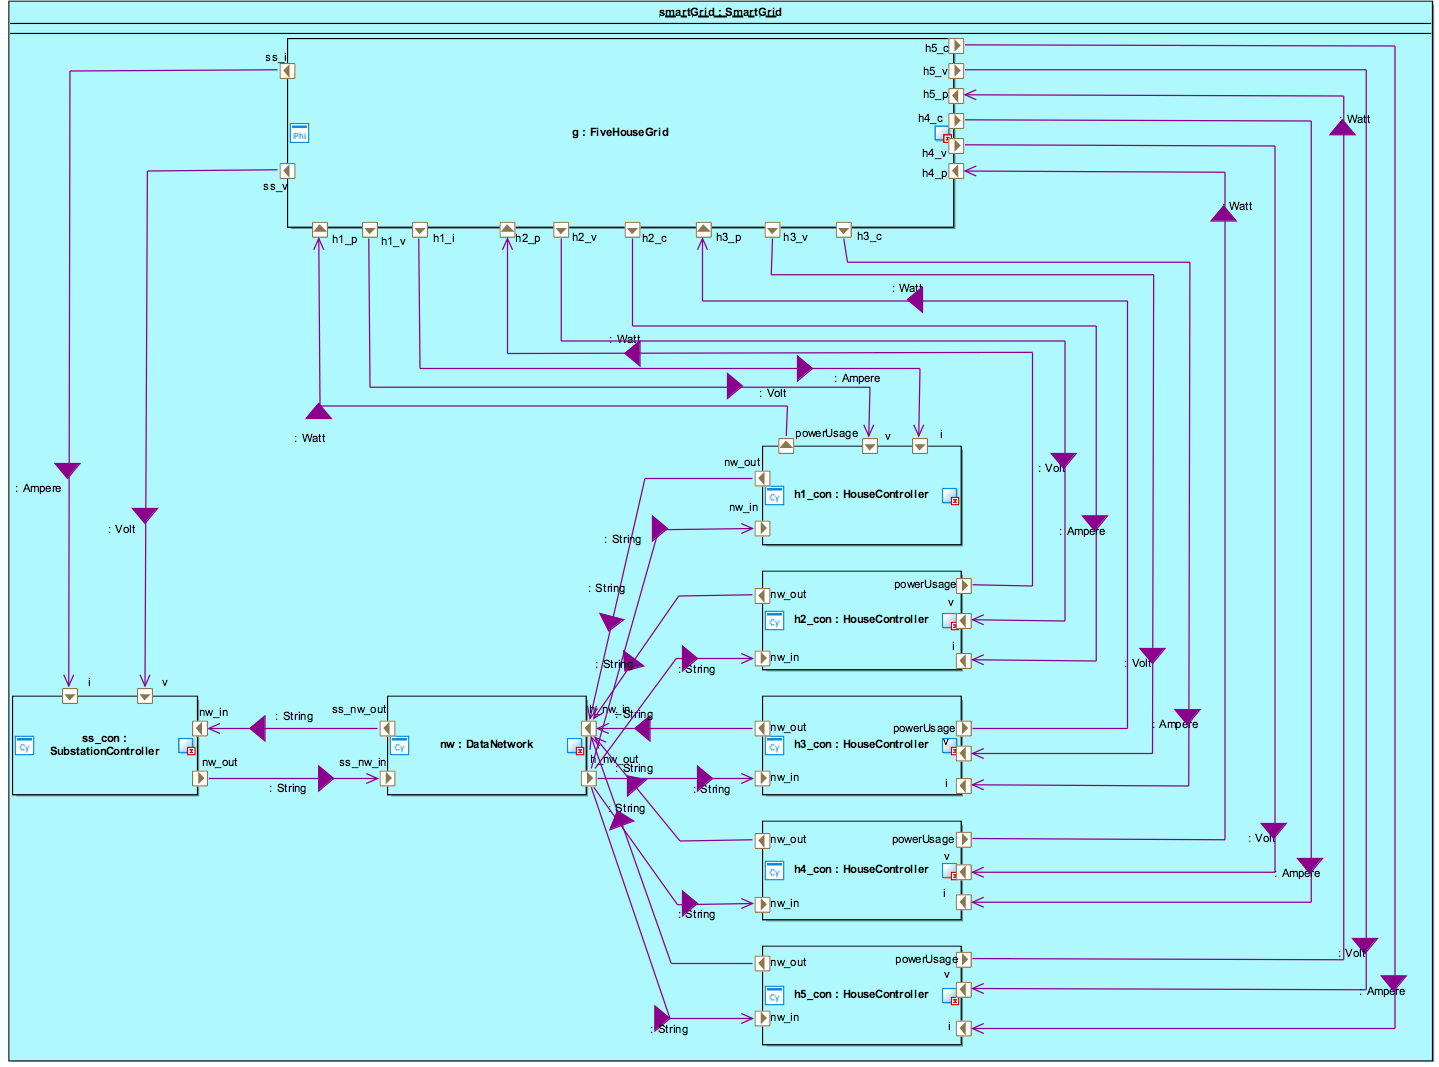
\includegraphics[width=1\textwidth]{smartgrid/5house_cd.png}
\caption{Connection Diagram for \SG multi-model}
\label{fig:cd_1h}
\end{center}
\end{figure}

It should be noted, in Deliverable D3.1a~\cite{INTOCPSD31a}, we presented two SysML models for a Smart Grid CPS. In these models we split the \emph{FiveHouseGrid} into a collection of separate EComponents to represent the different subparts of the physical infrastructure. At present, this is not feasible due to constraints on algorithmic loops formed between the elements. We will continue developing this in Year 3 of the project.

\subsection{Multi-model}
\label{sec:smartgrid_into_mm}

\subsubsection{Models}

The \SG\ multi-model comprises four `simulation' models: a single 20-sim model corresponding to the electrical grid and three VDM models for the substation controller, house controller and data network.

As alluded to in Section~\ref{sec:smartgrid_into_sys}, the physical aspects of the \SG \ CPS is contained in a single physical model. The use of bonds to connect the various internal elements (such as \emph{Power Generation}, \emph{Transmission} and \emph{Step-down Transformer}) limits the ability to spilt the physical model into smaller models. 

\begin{description}

\item[FiveHouseGrid:]

In the CT model we begin by defining a top-level block diagram in the 20-sim tool. This allows the composition of a model in terms of the different physical elements of the \SG\ CPS, and also to identify connections to the DE controller. This is shown in Figure~\ref{fig:20sim-sos}. It is important to note that in 20-sim, we model both \emph{effort} and \emph{flow} -- corresponding to \emph{voltage} and \emph{current} as we are modelling the electrical domain.


\begin{figure}[htb]
\begin{center}
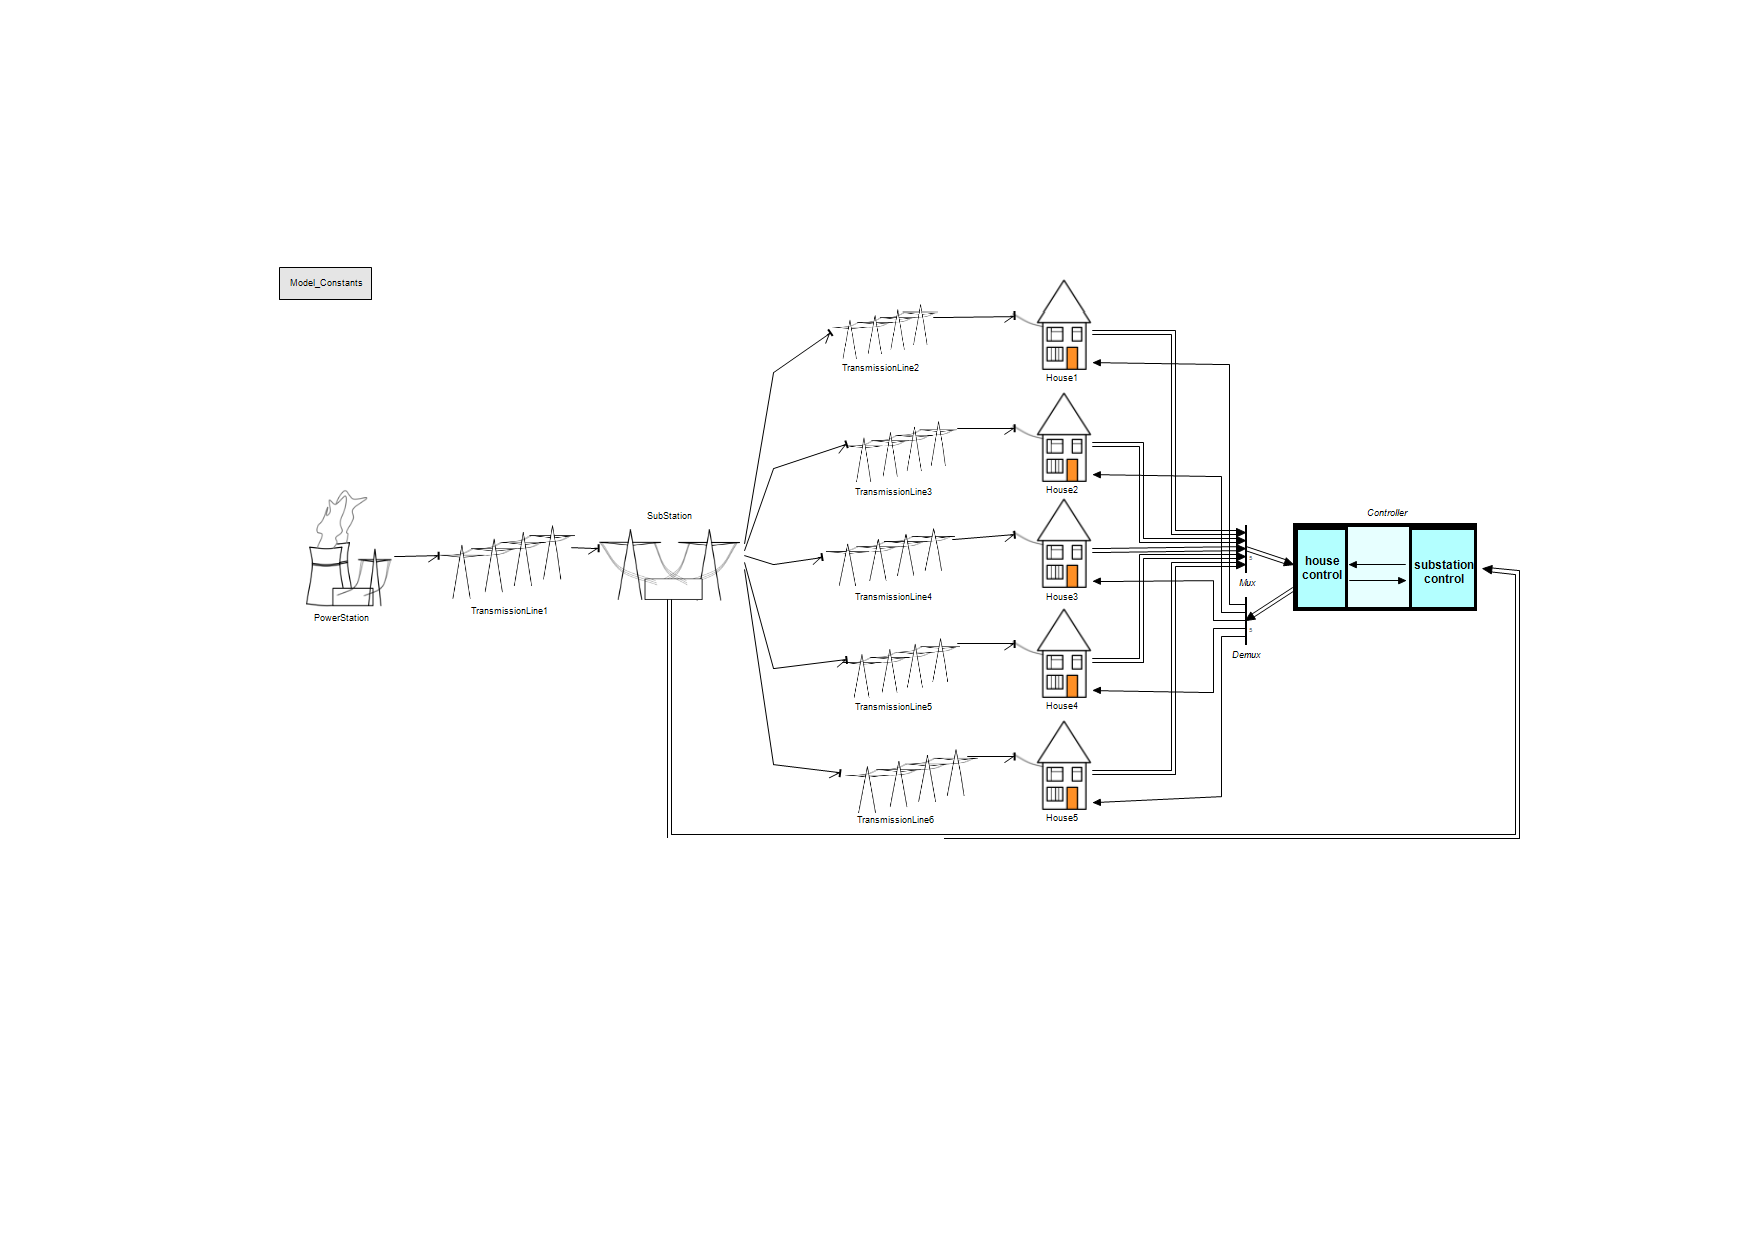
\includegraphics[width=0.8\textwidth]{smartgrid/20-sim-sos.pdf}
\caption{Top-level 20-sim block diagram connected by signals and energy bonds}
\label{fig:20sim-sos}
\end{center}
\end{figure}


The top-level block diagram is subsequently decomposed into different physical constituent elements: \textit{Power Generation}, \textit{Transmission Lines}, \textit{Substation} and \textit{Houses}. Each of these 20-sim blocks is given a graphical icon and may be `exploded' to show their internal structure in terms of 20-sim elements.

Defining the \textit{Power Generation} in Figure~\ref{fig:20sim-powergen}, we take an abstract view, comprising; a source of effort (\texttt{SE} in the model) representing a constant power source. For the purposes of this model, the voltage (effort) is defined as being 11000 volts.


\begin{figure}[htb]
\begin{center}
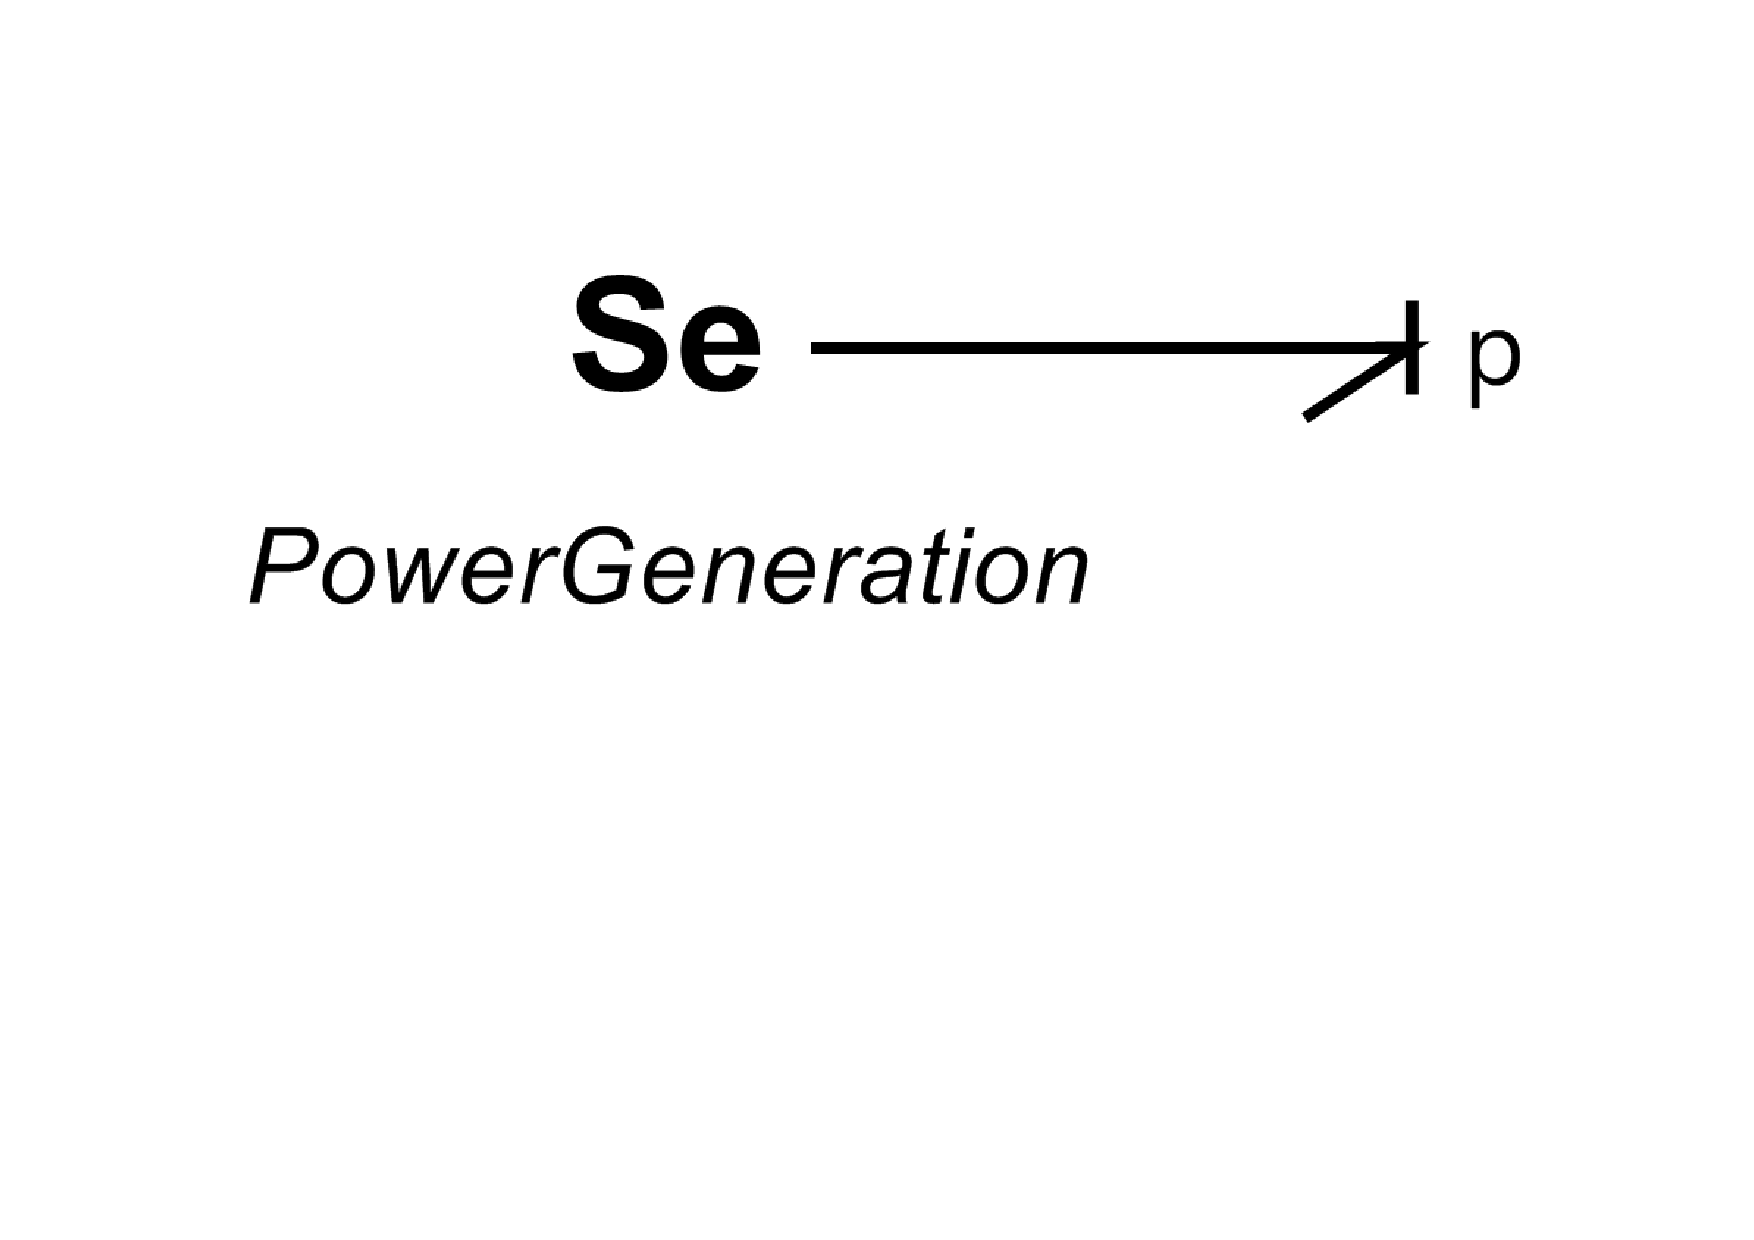
\includegraphics[width=0.2\textwidth]{smartgrid/20-sim-powergen.pdf}
\caption{20-sim elements comprising the Power Generation}
\label{fig:20sim-powergen}
\end{center}
\end{figure}

The \textit{Transmission Line}, shown in Figure~\ref{fig:20sim-transmission} is modelled simply as a resistor -- corresponding to the power drop experienced over such transmission lines. The resistance defined for the \textit{Transmission Lines} differs between the high voltage line between \textit{Power Generation} and \textit{Substation} and the lower voltage \textit{Transmission Line} between the \textit{Substation} and the \textit{Houses}.


\begin{figure}[htb]
\begin{center}
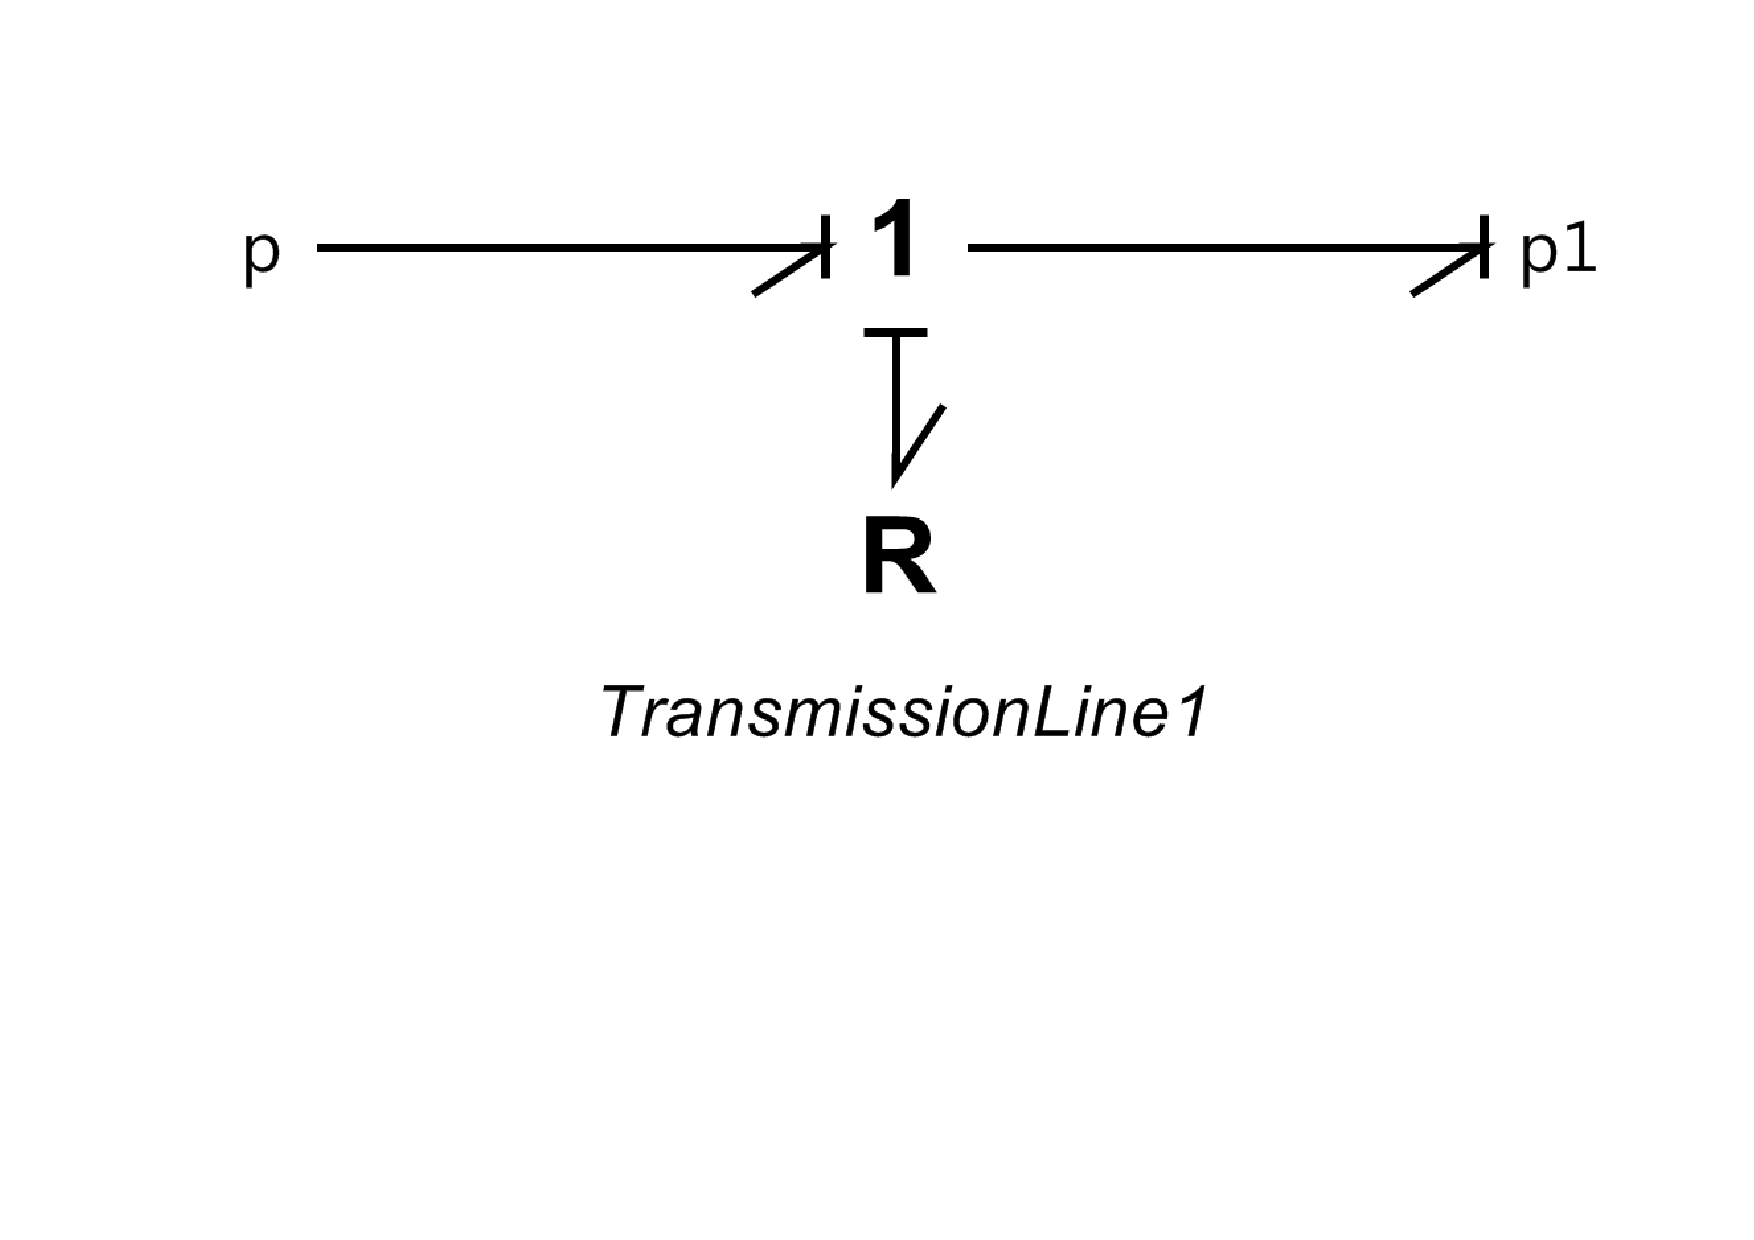
\includegraphics[width=0.3\textwidth]{smartgrid/20-sim-transmission.pdf}
\caption{20-sim elements comprising the Transmission Lines}
\label{fig:20sim-transmission}
\end{center}
\end{figure}

A \textit{Substation}, shown in Figure~\ref{fig:20sim-substation}  and as defined in the SysML architectural model, has two physical parts. Firstly, the \textit{Step-down Transformer} alters the voltage from the high transmission voltage to the target local voltage of 230 volts. The \textit{Substation Meter} is modelled as a smart meter, in Figure~\ref{fig:20sim-meter} using \emph{effort} and \emph{flow meters} (an `e' and `f' surrounded by a circle) to monitor the voltage and current observed in the substation.

\begin{figure}[htb]
\begin{center}
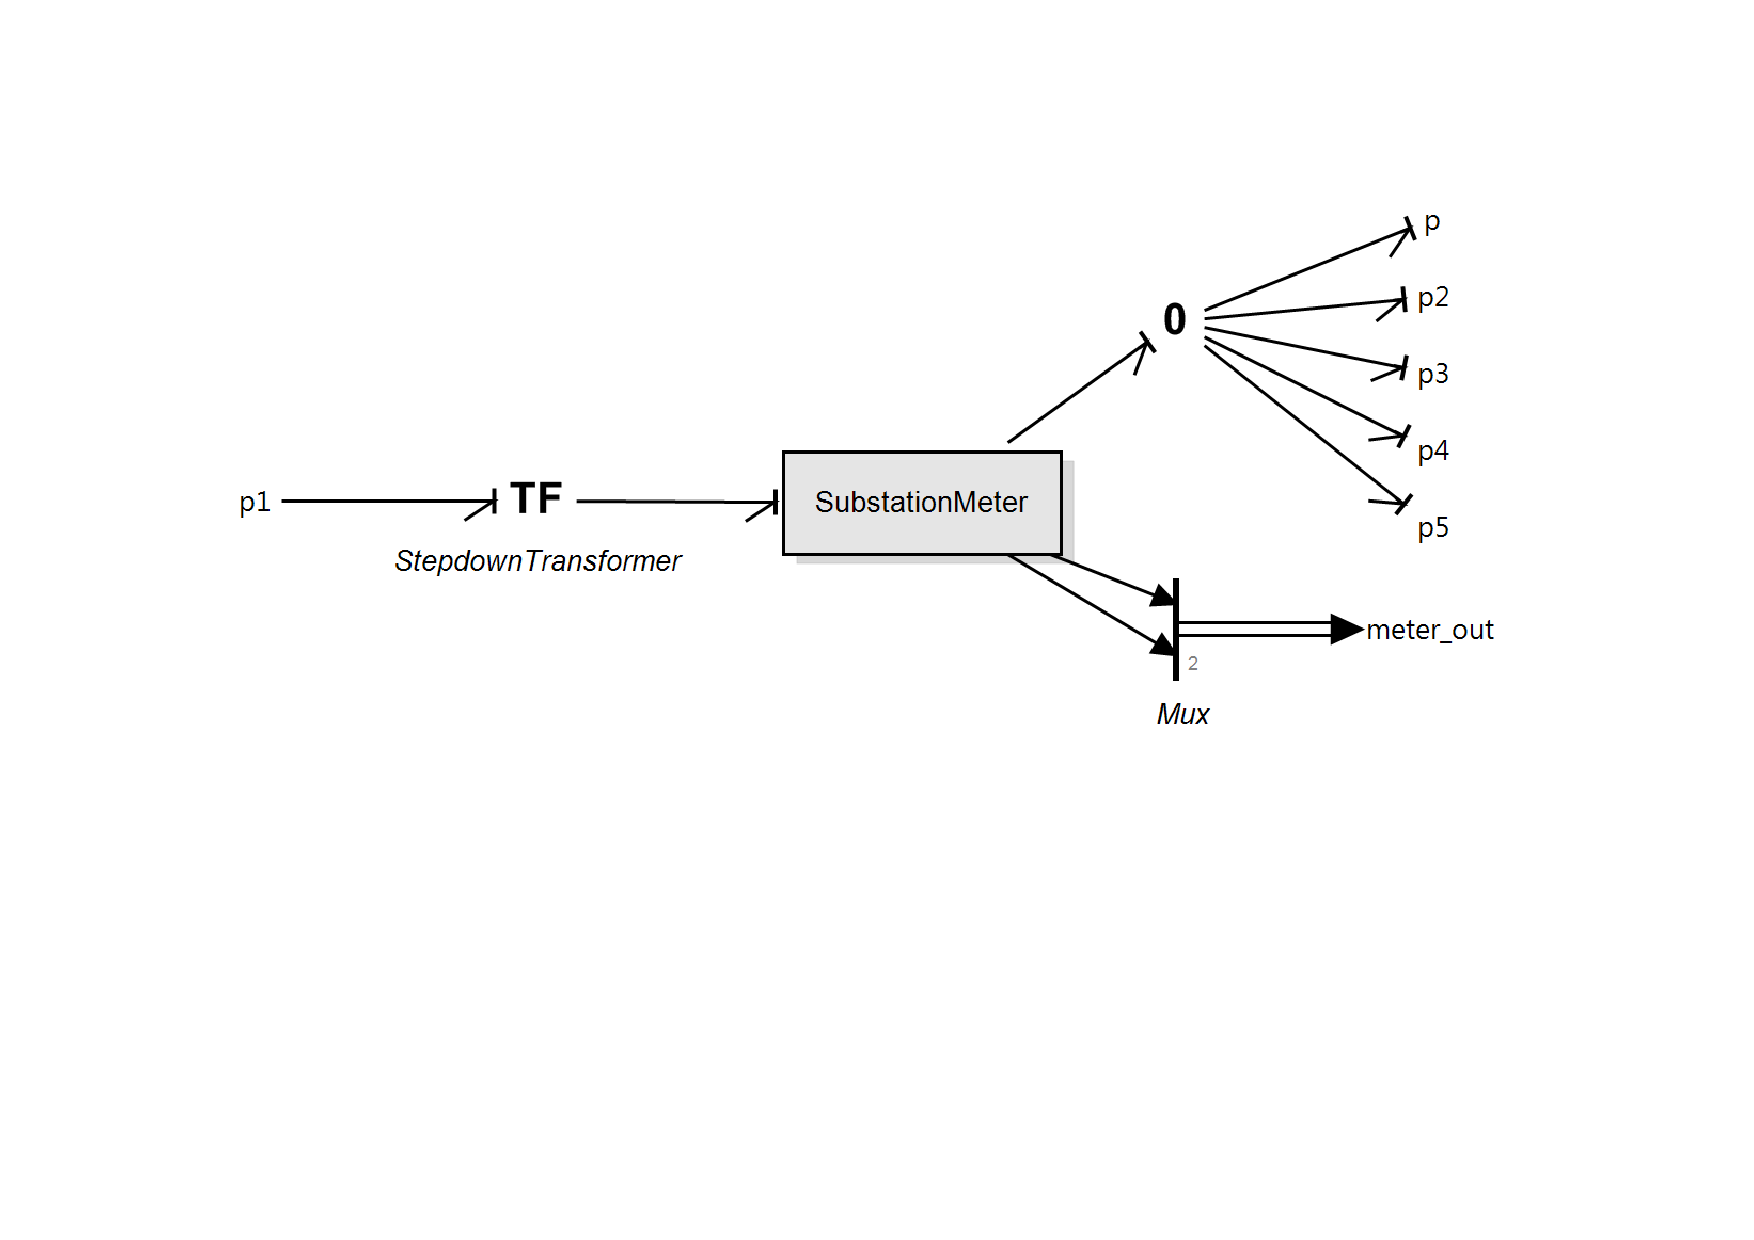
\includegraphics[width=0.7\textwidth]{smartgrid/20-sim-substation.pdf}
\caption{20-sim elements comprising the Substation}
\label{fig:20sim-substation}
\end{center}
\end{figure}

\begin{figure}[htb]
\begin{center}
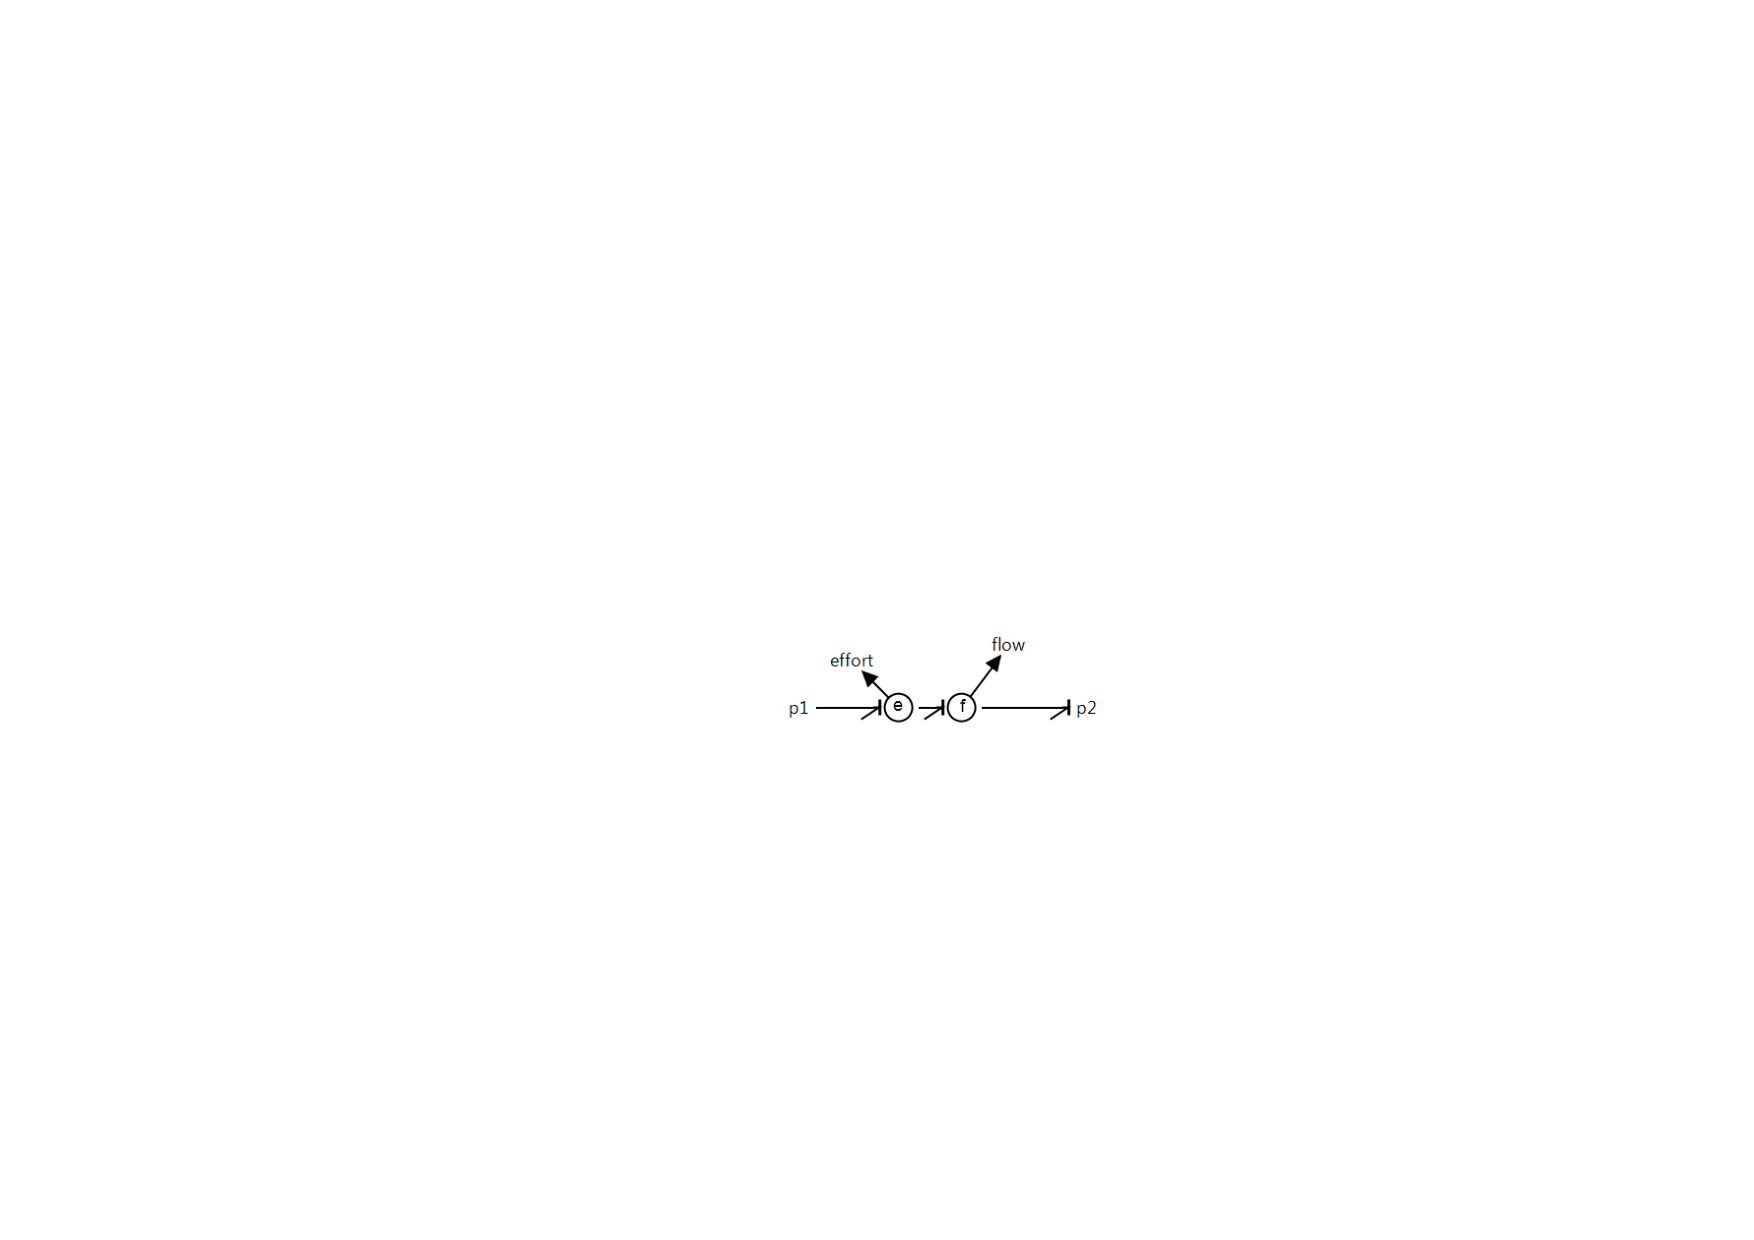
\includegraphics[width=0.4\textwidth]{smartgrid/20-sim-meter.pdf}
\caption{20-sim elements comprising a Smart Meter}
\label{fig:20sim-meter}
\end{center}
\end{figure}

Finally, the \textit{Houses}, shown in Figure~\ref{fig:20sim-house}, are each modelled as containing a \textit{House Meter} and a set of devices. The \textit{House Meters} are modelled in the same way as the \textit{Substation Meter}. The \textit{Devices} are defined as being a variable resistor. The resistance is calculated using a variable \emph{powerUsage}. This value is provided by a source external to the model.

\begin{figure}[htb]
\begin{center}
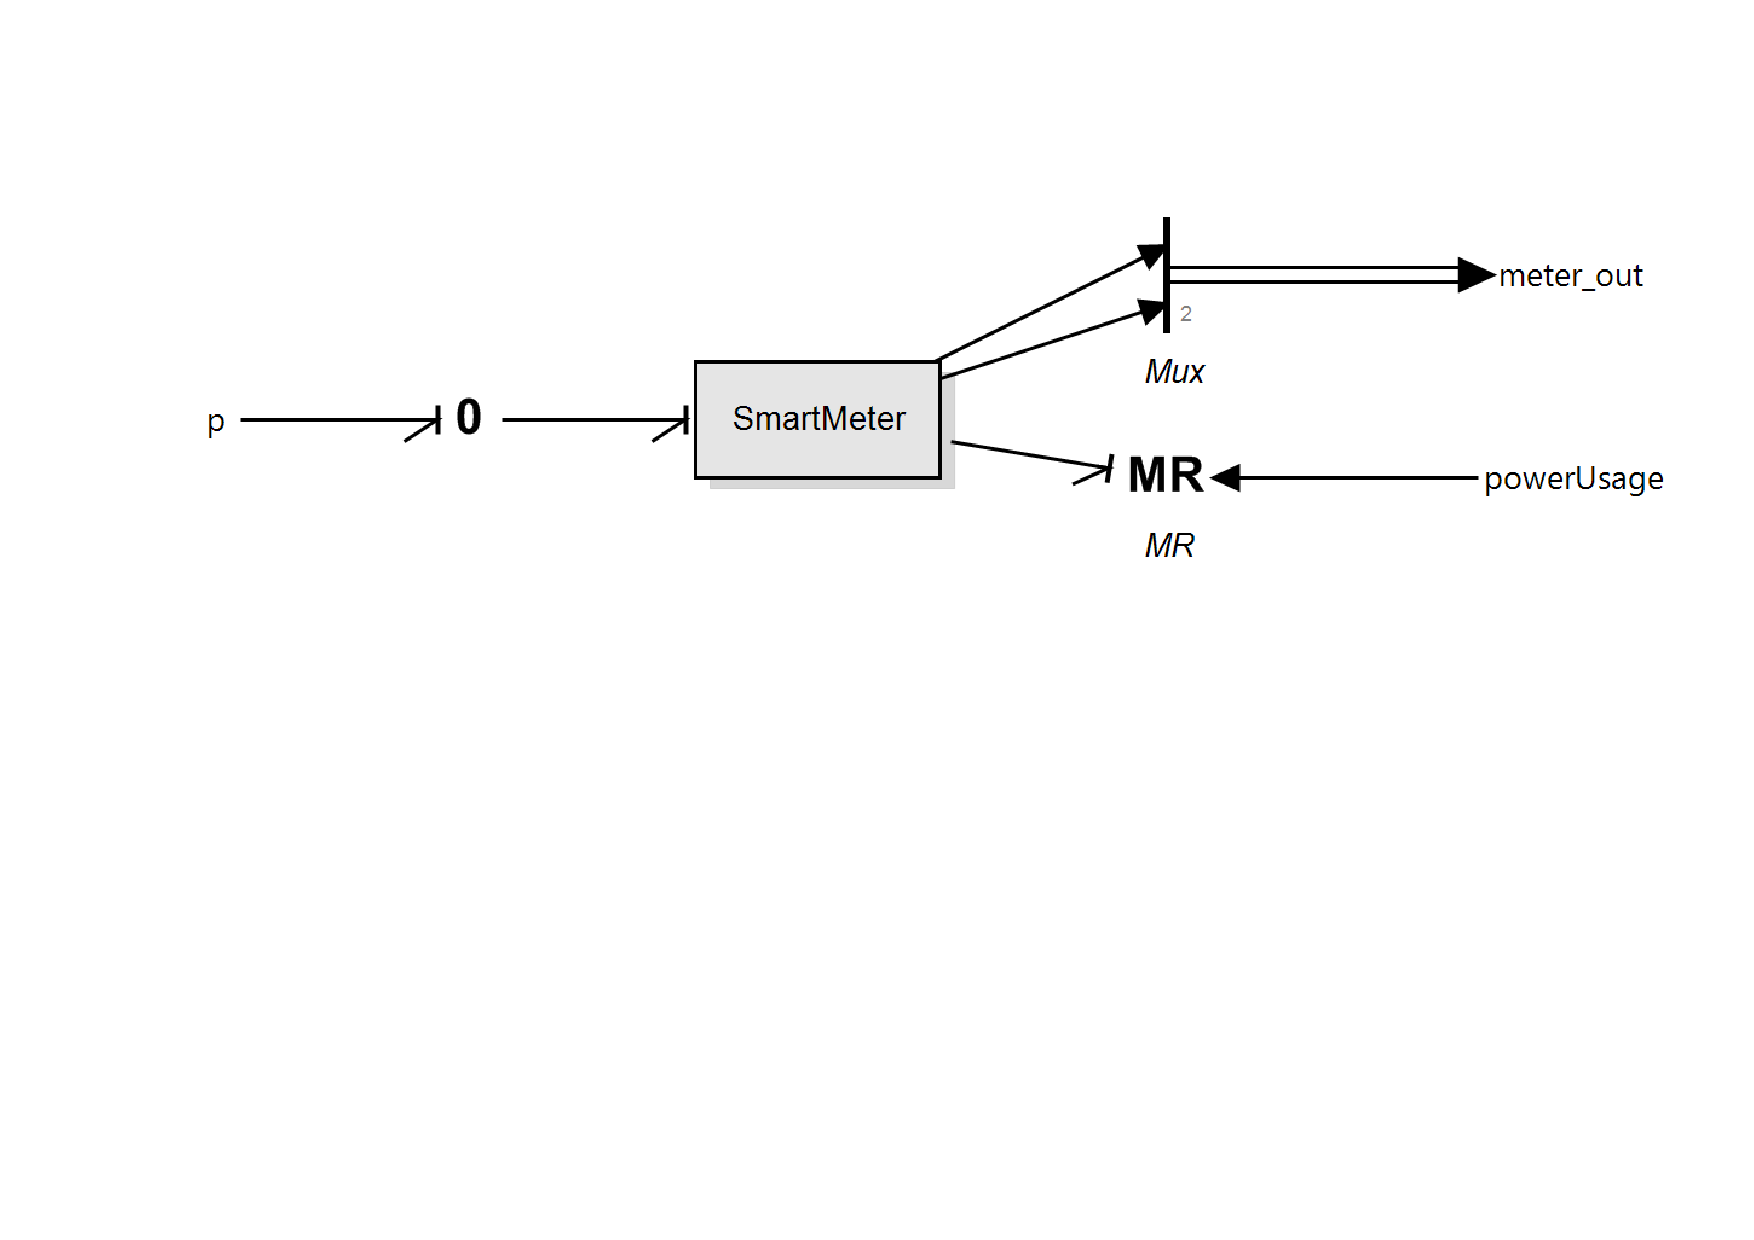
\includegraphics[width=0.7\textwidth]{smartgrid/20-sim-house.pdf}
\caption{20-sim elements comprising a House}
\label{fig:20sim-house}
\end{center}
\end{figure}

The final 20-sim artefact to consider is the link to the DE controller. This element receives an array input (the voltage and current provided by the \textit{Substation Meter}) and a matrix of \textit{House Meter} readings (again voltage and current). The controller returns an array of values corresponding to the power usage of the different houses. The software controller itself is defined in a VDM-RT model, described in the next section.

\item[HouseController] The \emph{HouseController} VDM-RT model dictates, and aims to manage, the power usage of each house. The power usage takes two forms: unmanaged profiles of usage -- where devices are used solely at the behest of the user; and managed power use -- where the controller may manage the power use. The architecture is shown in Figure~\ref{fig:vdm-house}. The \emph{System} class contains an instance of the \emph{Controller}, \emph{HardwareInterface} and \emph{IOFactory} classes. The \emph{HardwareInterface} class contains input and output ports for the model -- communication with the \emph{FiveHouseGrid} model (inputs are the house voltage and current, with the house power usage as output), and with the \emph{DataNetwork} (with input and outputs for data communication).

\begin{figure}[htb]
\begin{center}
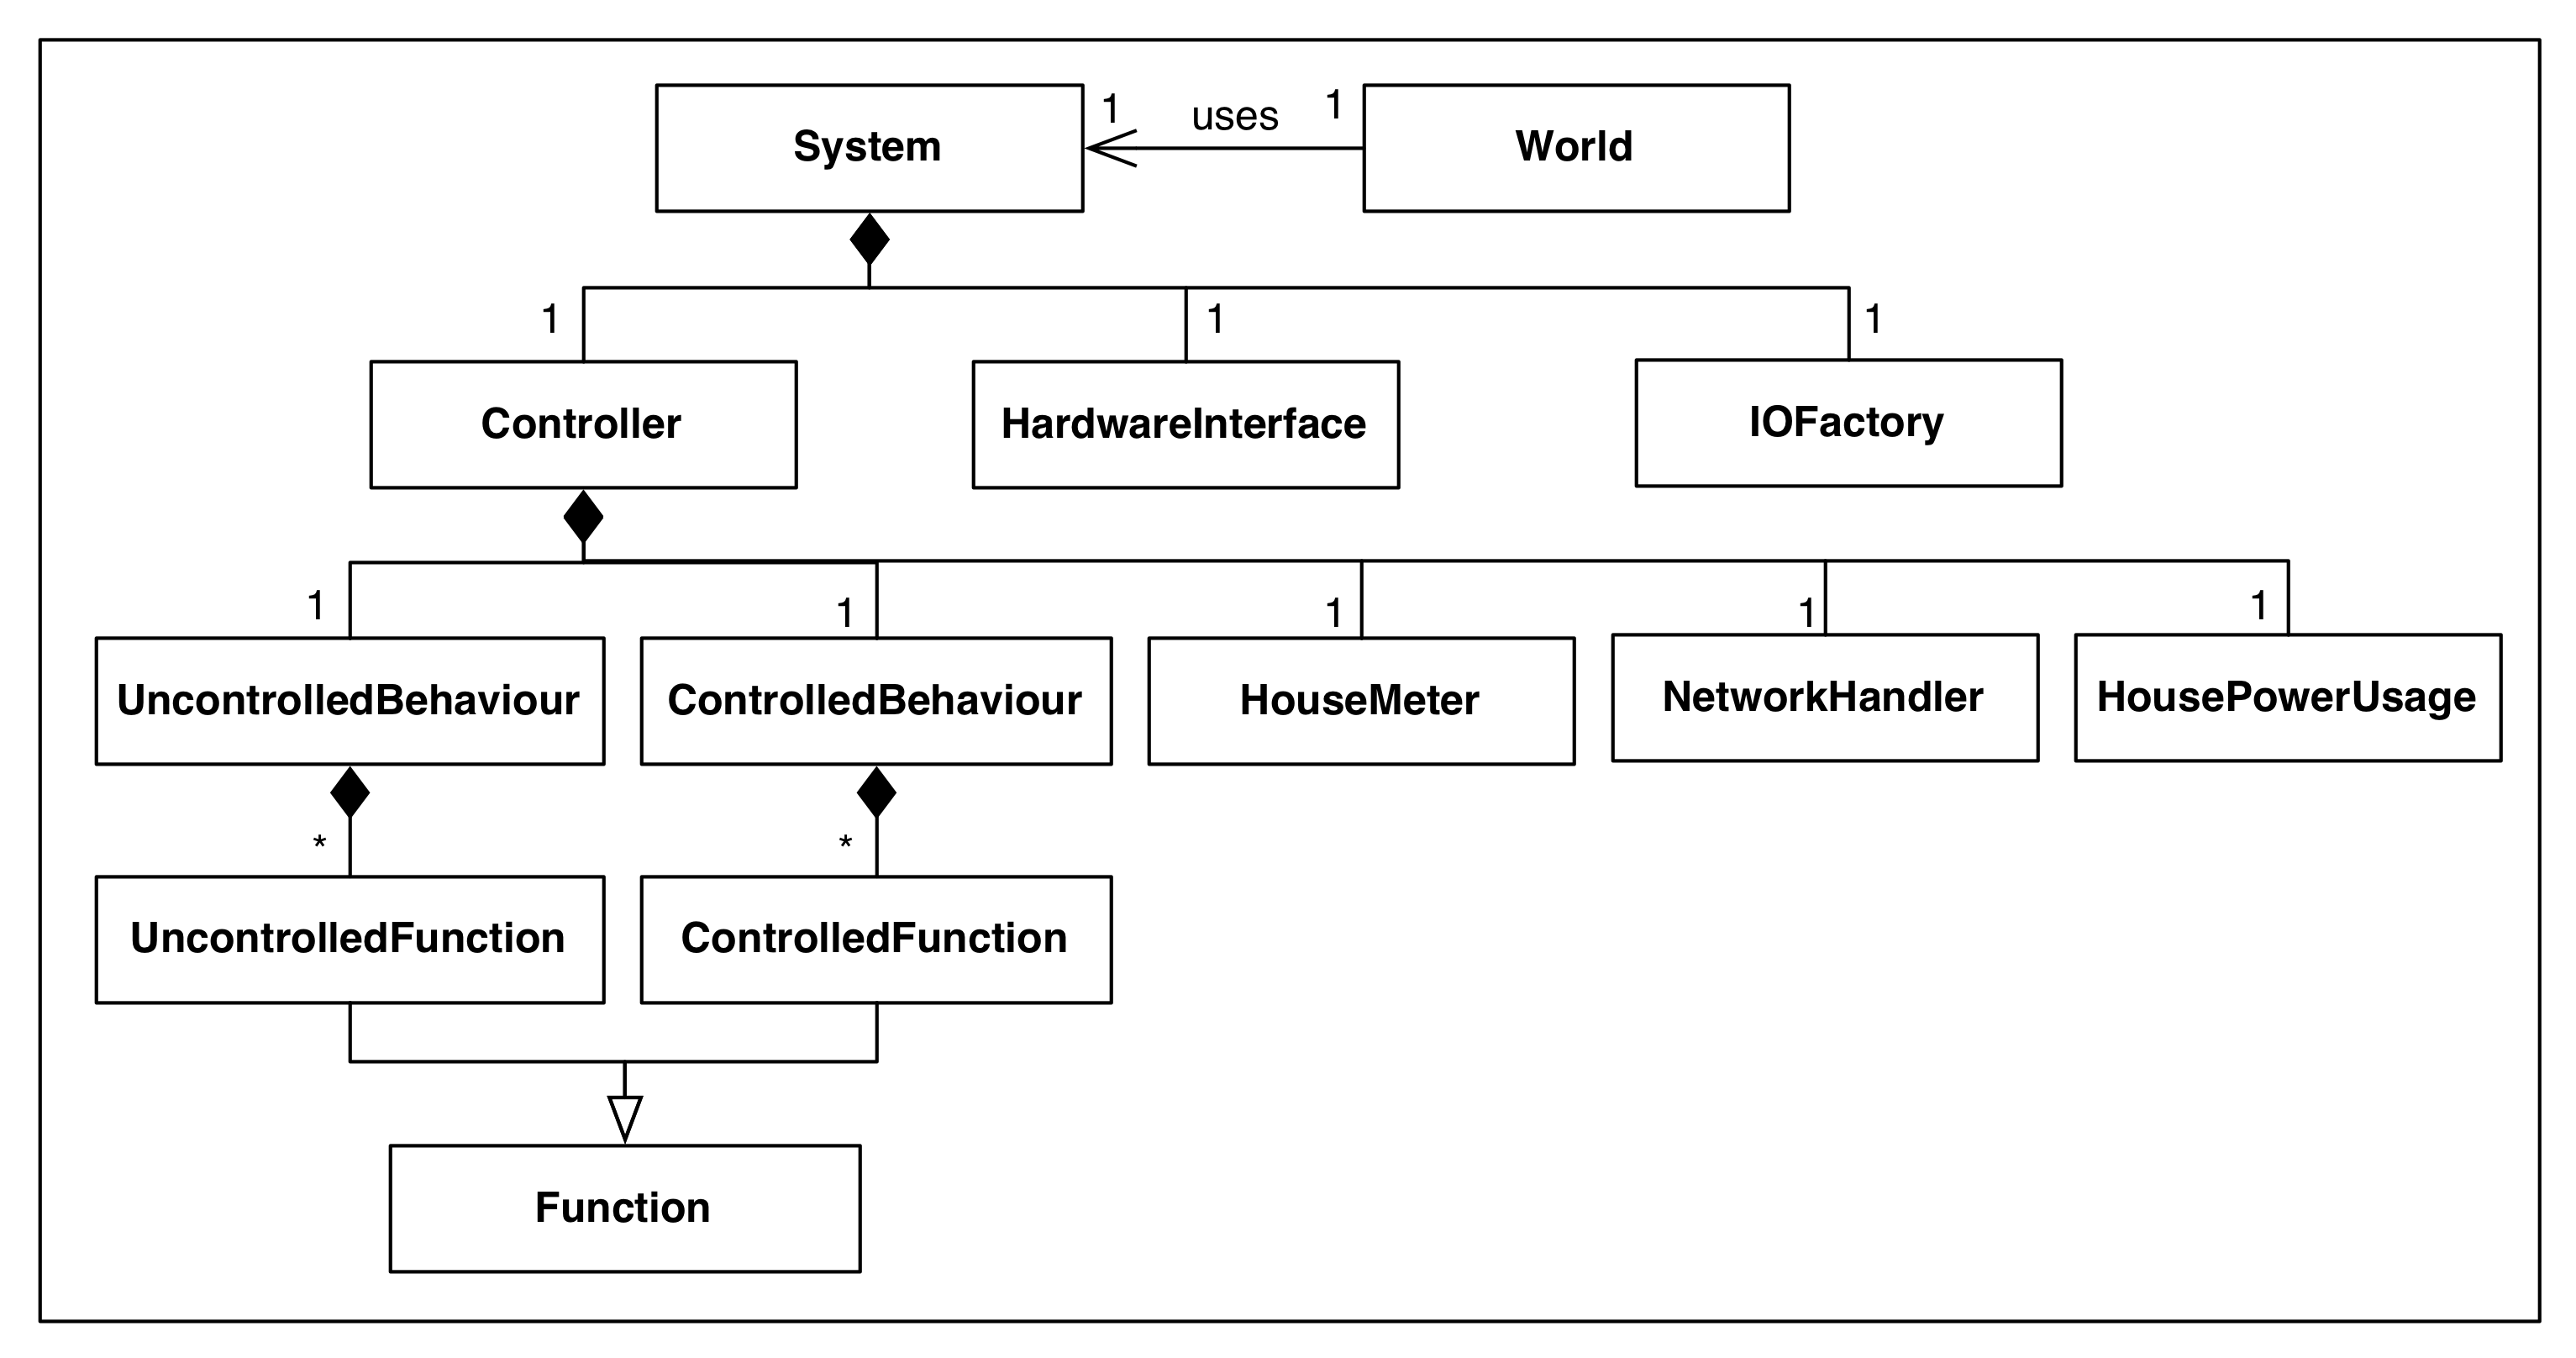
\includegraphics[width=0.8\textwidth]{smartgrid/housecontrollerarch}
\caption{Architecture of HouseController model}
\label{fig:vdm-house}
\end{center}
\end{figure}

In the case of unmanaged power usage, this may mean that the home owner turns devices and appliances on and off at will, or where some appliances change power usage at set times through the day (heating, for example). In the VDM-RT model, we define a collection of appliance and device power use profiles, a map of time to power use, which will always occur during simulation. Each house is initialised with a collection of device power profiles.

Managed power sources are modelled in a similar manner to unmanaged sources, apart from the fact they have a shorter profile, and no fixed start time. The HouseController may, therefore, change the start time of a managed device depending upon a policy defined in the controller. At present, once a device has started, it can not be paused, however this may be changed in future.

The HouseController has several control mechanisms for managing the controlled devices in that household. These include:
\begin{description}
\item[No controlled devices:] In this mode the house controller cancels all controllable devices from starting. This can be reversed, however at present if the start time passes whilst cancelled, the device will not turn on in the future. This mode does not stop already running devices.

\item[No management:] The controlled devices operate as requested -- the controller does not alter the start time.

\item[Local control:] The decision to start a controlled device is based upon the local meter readings at a set time before the device is scheduled to start. Each house has a voltage threshold -- which dictates the minimum voltage permitted for a smart device to be turned on. If the voltage is below this threshold, the starting time of the smart device is increased by a set time.

\item[Request:] The HouseController makes an explicit request to the substation to check if controlled devices may start.

%\item[Consensus:] This is equivalent to fully distributed control, and has not yet been implemented. This is a complex problem, beyond the scope of this project.
%
%\item[Substation control:] In this mode, the SubstationController manages the controlled devices with no input from the HouseController.
\end{description}

Additional control mechanisms may be added at a later time.

\item[SubstationController:] The \emph{SubstationController} VDM-RT model architecture is shown in Figure~\ref{fig:vdm-ss}. The SubstationController aims to manage the power across a set of houses. The controller takes, as input, the voltage and current at the substation and also receives meter readings from all the houses it is managing. A network may be modelled for the transmission of these readings, allowing for the modelling of a faulty network. In this project we abstract from the network and assume a perfect network.

The SubstationController is able to make decisions and influence the behaviour of the individual HouseControllers based upon the meter reading values at any point. The SubstationController has two control mechanisms available to a policy designer:


\begin{description}
\item[Reporting:] This is the simplest mode, whereby it receives readings from each of the houses but takes no action. In this mode, however, the SubstationController may still respond to requests made by the different HouseControllers.

\item[Substation control:] In this mode, the SubstationController takes control of controlled devices of all houses in the neighbourhood. Modelling this is beyond the scope of the project, however we could envisage multiple subtypes of this control mode depending on how the engineer decides upon which devices to allow to start, for example depending on financial incentives.
\end{description}


\begin{figure}[htb]
\begin{center}
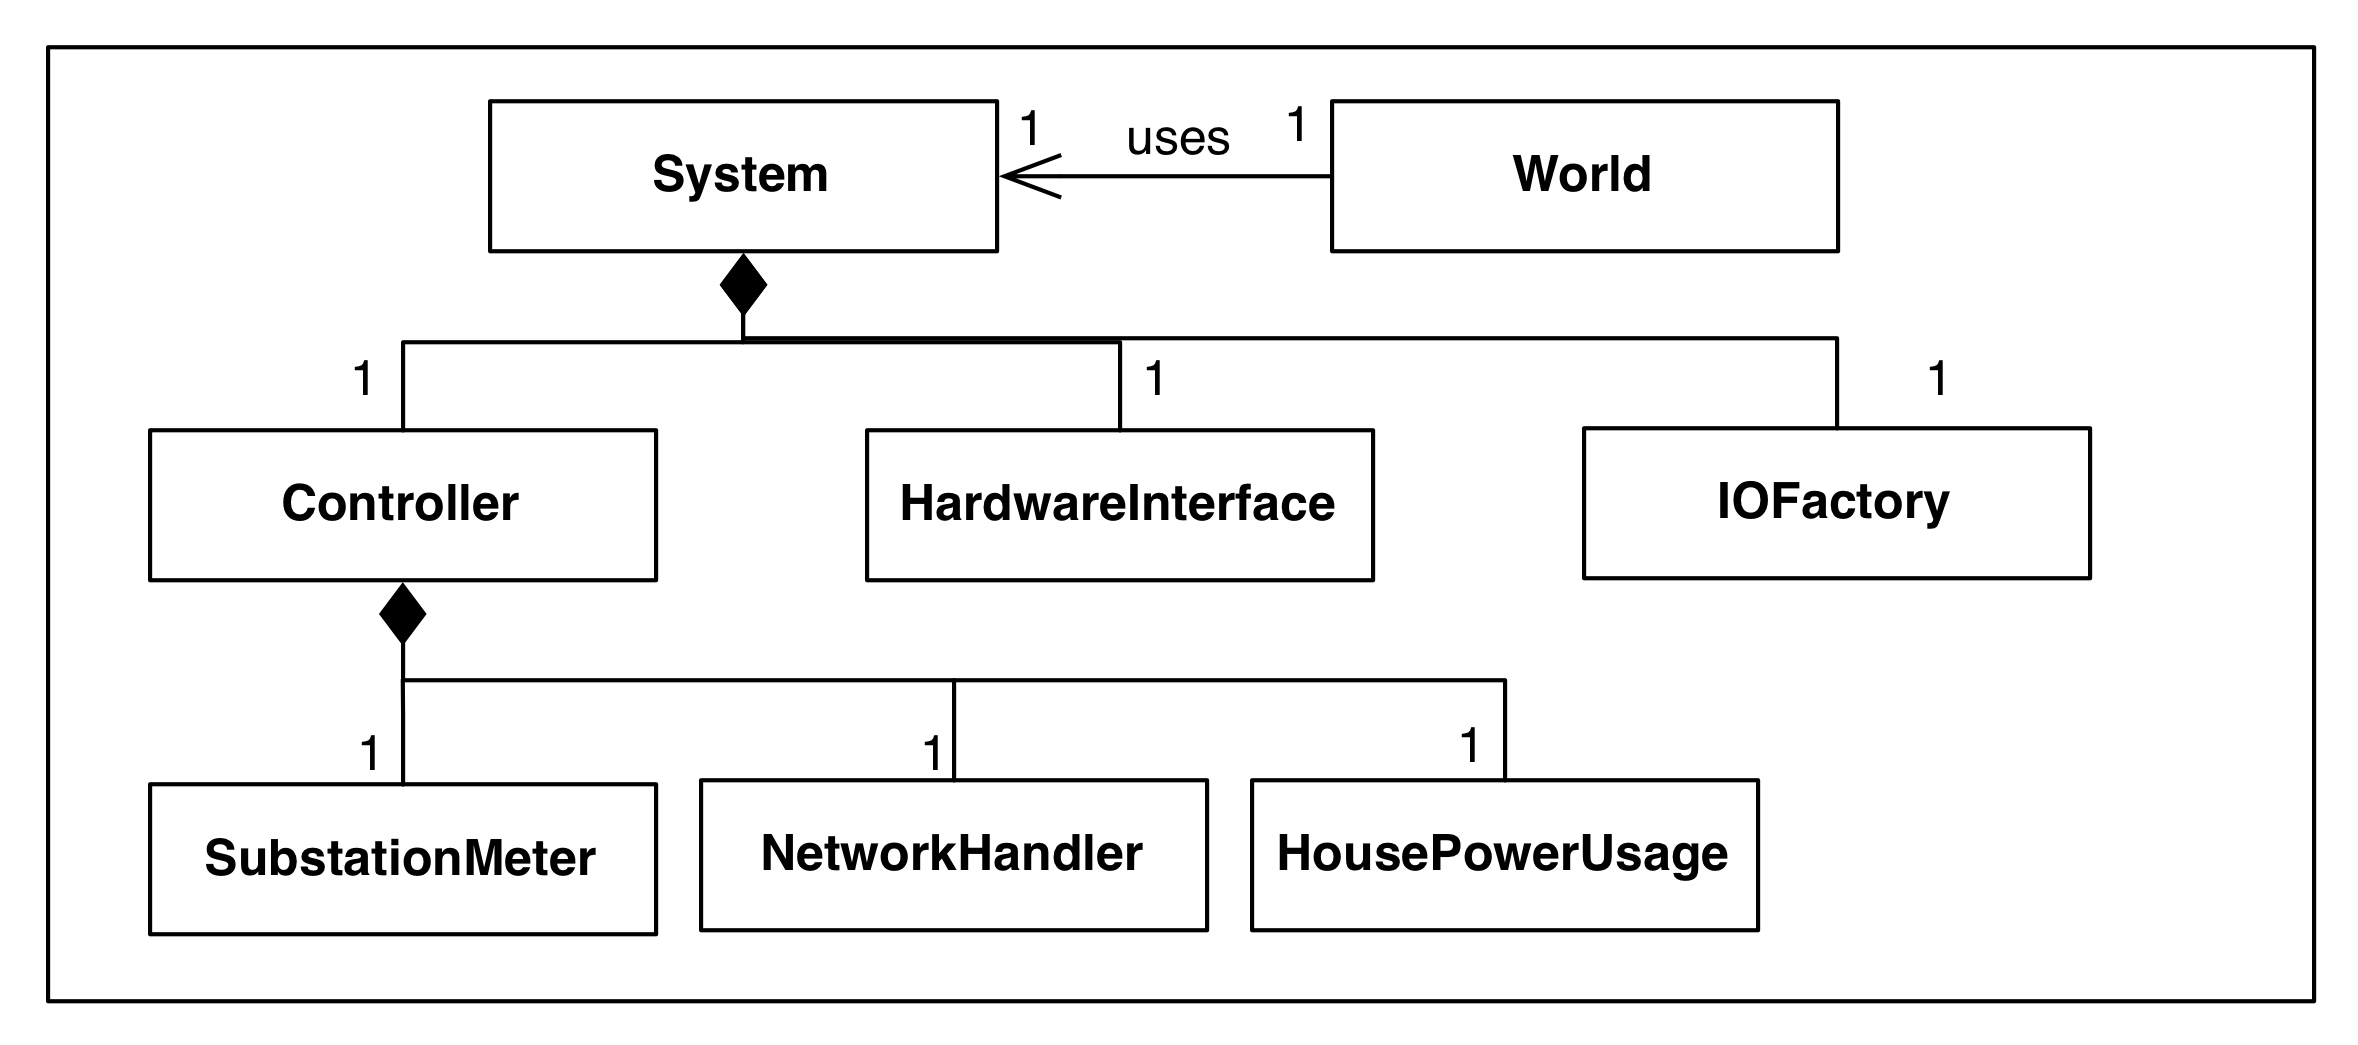
\includegraphics[width=0.75\textwidth]{smartgrid/sscontrollerarch}
\caption{Architecture of SubstationController model}
\label{fig:vdm-ss}
\end{center}
\end{figure}

\item[DataNetwork] Not yet defined -- in Year 3 of the project, we shall implement this model using the Ether pilot study -- see Section~\ref{sec:ether}.

\end{description}



\subsubsection{Configuration}

In this pilot, we see four groups of connections.

The first, between the physical \emph{FiveHouseGrid} and the cyber \emph{SubstationController}, relate to the metering of voltage and current at the substation of the grid. The connections are:

\begin{itemize}
  \item from the \emph{FiveHouseGrid} \texttt{ss\_i} port to the \emph{SubstationController} \texttt{i} port, and
  \item from the \emph{FiveHouseGrid}  \texttt{ss\_v} port to the \emph{SubstationController} \texttt{v} port.
\end{itemize}

Next, connections exist between the physical \emph{FiveHouseGrid} and the each of the five cyber \emph{HouseControllers}, relating to the metering of voltage and current at the substation of the grid. In addition, there is a connection carrying the current power usage commands from the controller to the grid. Due to the number of connections, we consider only one house instance here. The connections are:

\begin{itemize}
  \item from the \emph{FiveHouseGrid} \texttt{h\_i} port to the \emph{HouseController} \texttt{i} port, 
  \item from the \emph{FiveHouseGrid} \texttt{h\_v} port to the \emph{HouseController} \texttt{v} port, and
  \item from the \emph{HouseController}  \texttt{powerUsage} port to the \emph{FiveHouseGrid} \texttt{h\_p} port.
\end{itemize}

The next collection contains two connections between the \emph{DataNetwork} and \emph{SubstationController} to represent the flow of data into and out of the \emph{SubstationController}.

\begin{itemize}
  \item from the \emph{DataNetwork} \texttt{ss\_nw\_out} port to the \emph{SubstationController} \texttt{nw\_in} port, and
  \item from the \emph{SubstationController}  \texttt{nw\_out} port to the \emph{DataNetwork} \texttt{ss\_nw\_in} port.
\end{itemize}

Finally, we present two connections between the \emph{DataNetwork} and \emph{HouseController} to represent the flow of data into and out of the \emph{HouseController}. Again, we consider only one house instance here.

\begin{itemize}
  \item from the \emph{DataNetwork} \texttt{h\_nw\_out} port to the \emph{HouseController} \texttt{nw\_in} port, and
  \item from the \emph{HouseController}  \texttt{nw\_out} port to the \emph{DataNetwork} \texttt{h\_nw\_in} port.
\end{itemize}

\subsection{Co-simulation}
\label{sec:smartgrid_into_co}

FMUs have not yet been generated from the models of this study and therefore co-simulation has not yet been performed. This shall follow in Year 3 of INTO-CPS.

%\subsubsection{Analyses and Experiments}
%\label{sec:smartgrid_into_analysis}
